\documentclass[a4paper,12pt]{article}
\usepackage[english,ukrainian,russian]{babel}
\linespread{1}
\usepackage{ucs}
\usepackage[utf8]{inputenc}
\usepackage[T2A]{fontenc}
\usepackage[paper=portrait,pagesize]{typearea}
\usepackage{amsmath}
\usepackage{bigints}
\usepackage{amsfonts}
\usepackage{graphicx}
\usepackage{amssymb}
\usepackage{cancel}
\usepackage{gensymb}
\usepackage{multirow}
\usepackage{rotate} 
\usepackage{pdflscape}
\usepackage{bigstrut}
\usepackage[pageanchor]{hyperref}
\usepackage{chngpage}
\usepackage{fancybox,fancyhdr}
\newcommand\tab[1][1cm]{\hspace*{#1}}
\newcommand{\RomanNumeralCaps}[1]{\MakeUppercase{\romannumeral #1}}
\usepackage[left=20mm, top=20mm, right=15mm, bottom=15mm, nofoot]{geometry}

\usepackage{verbatim}
\usepackage{enumerate}
\usepackage{listings}
\usepackage{xcolor}

\definecolor{codegreen}{rgb}{0,0.6,0}
\definecolor{codegray}{rgb}{0.5,0.5,0.5}
\definecolor{codepurple}{rgb}{0.58,0,0.82}
\definecolor{backcolour}{rgb}{0.95,0.95,0.92}

\lstdefinestyle{mystyle}{
	backgroundcolor=\color{backcolour},   
	commentstyle=\color{codegreen},
	keywordstyle=\color{blue},
	numberstyle=\tiny\color{codegray},
	stringstyle=\color{red},
	basicstyle=\ttfamily\footnotesize,
	breakatwhitespace=false,         
	breaklines=true,                 
	captionpos=b,                    
	keepspaces=true,                 
	numbers=none,                    
	numbersep=5pt,                  
	showspaces=false,                
	showstringspaces=false,
	showtabs=false,                  
	tabsize=4,
	frame=shadowbox
}

\lstset{style=mystyle}

% Language "Assembler"
\lstdefinelanguage{assembler}{
    keywords={mov, add, sub, mul, div, jmp, cmp, jne, je, push, pop, call, ret},
    sensitive=true,
    comment=[l]{;},  % Коментарі починаються з ;
    morestring=[b]",  % Рядки в лапках
    morestring=[b]',  % Рядки в одинарних лапках
}
\lstset{
    language=assembler,      % Встановлюємо мову
    basicstyle=\ttfamily,    % Шрифт для коду
    keywordstyle=\color{blue},    % Стиль для ключових слів
    commentstyle=\color{codegreen},    % Стиль для коментарів
    stringstyle=\color{red},    % Стиль для рядків
    numbers=left,          % Номери рядків зліва
    numberstyle=\tiny,     % Стиль номерів рядків
    stepnumber=0,         % Номери для кожного рядка
    numbersep=5pt,        % Відстань до номера рядка
    frame=single,         % Рамка навколо коду
}

\begin{document}
    \pagestyle{fancy}
    \fancyhead{}
    \fancyhead[R]{ФІ-12 Завалій Олександр}
    \begin{center}
        \large{\textbf{Міністерство освіти і науки України\\
                Національний технічний університет України\\
                «Київський політехнічний інститут імені Ігоря Сікорського»\\
                Навчально-науковий Фізико-технічний інститут}}\\
        \hfill \break \hfill \break \hfill\break \hfill \break \hfill \break \hfill \break \hfill \break
        \hfill \break \hfill \break \hfill \break
        \begin{center}
            \normalsize{\textbf{Архітектура комп'ютерних систем\\
            Комп’ютерний практикум\\
            Робота №2}}
        \end{center}
    \end{center}
    \hfill \break \hfill \break \hfill \break \hfill \break \hfill \break \hfill \break \hfill \break
    \hfill \break \hfill \break \hfill \break \hfill \break 
    \begin{flushright}
        \large{ \hspace{35pt} Виконав:\\
            студент групи ФI-12\\
            Завалій Олександр\\} 
        \large{ \hspace{35pt} Перевірив:\\
        Козленко О.В.} 
    \end{flushright}
    \hfill \break \hfill \break \hfill \break \hfill \break \hfill \break \hfill \break \hfill \break
    \hfill \break
    \begin{center} \textbf{Київ-2024} \end{center}
    \thispagestyle{empty}

\newpage
    \begin{center}
        \section*{\bfseries{Робота №2.\\
        Основи побудови програми на асемблері в архітектурі ІА-32
    }}
    \end{center}
    \textbf{Мета:} \\
    \hangindent=1.5cm 
    \hangafter=+1 \noindent
    Ознайомитися з створенням базової програми виключно на мові асемблер для платформи на архітектурі ІА-32 \\
    \begin{center}
        \Large{Варіант №4}
    \end{center}
    Зміст індивідуального завдання:
    \begin{enumerate}
        \item Визначити дані. \\
        $
        a(1)\rightarrow 8,\: 
        a(2)\rightarrow 5,\:
        a(3)\rightarrow 3,\:
        c1  \rightarrow 20,\:
        c2  \rightarrow 6$
        \item Занести в регістри такі величини. \\
        $
        AX\rightarrow a(1)+a(2)-a(3),\:
        BX\rightarrow a(1)\cdot a(2),\:
        CX\rightarrow c1-c2,\:
        DX\rightarrow ((c1\: \&\: a(2)),\: a(3))$
        \item Організувати цикл, послідовно зменшуючи число у регістрі $CX$ на $1$. У
        циклі зменшувати число, що знаходиться у регістрі $BX$ на величину, що
        знаходиться у регістрі $AX$, поки значення $CX$ не стане дорівнювати $0$.
    \end{enumerate}

\newpage
    \begin{center}
        \Large{Code}
    \end{center}
    Код на мові Assembler.
    \begin{lstlisting}[language=assembler]
section .bss
    val_AX resd 1
    val_BX resd 1
    val_CX resd 1
    val_DX resd 1

section .data
    a db 8, 5, 3
    c1 db 20
    c2 db 6
    fmt db "Result: %d", 10, 0

section .text
    extern printf
    global main

main:
    push ebp
    mov ebp, esp

    ; AX = a(1) + a(2) - a(3)
    mov al, [a]
    add al, [a+1]
    sub al, [a+2]
    movzx eax, al
    mov [val_AX], eax
    
    ; BX = a(1) * a(2)
    mov al, [a]
    mov bl, [a+1]
    movzx eax, al
    movzx ebx, bl
    imul eax, ebx
    mov [val_BX], eax

    ; CX = c1 - c2
    mov al, [c1]
    sub al, [c2]
    movzx eax, al
    mov [val_CX], eax
    
    ; DX = ((c1 & a(2)), a(3))
    mov al, [c1]
    and al, [a+1]
    add al, [a+2]
    movzx eax, al
    mov [val_DX], eax
    \end{lstlisting}

\newpage
    \begin{lstlisting}[language=assembler]
    ; Loop
    loop_start:
        mov eax, [val_CX]
        cmp eax, 0
        je loop_end

        ; CX = CX - 1
        sub dword [val_CX], 1

        ; BX = BX - AX
        mov eax, [val_BX]
        sub eax, [val_AX]
        mov [val_BX], eax
        jmp loop_start

    loop_end:
        push dword [val_BX]
        push fmt
        call printf
        add esp, 8

    leave
    ret
    \end{lstlisting}
    Для перевірки коректності обрахунків я написав код на мові Python.
    \begin{figure}[h!]
        \begin{minipage}[h]{1\linewidth}
            \centering
            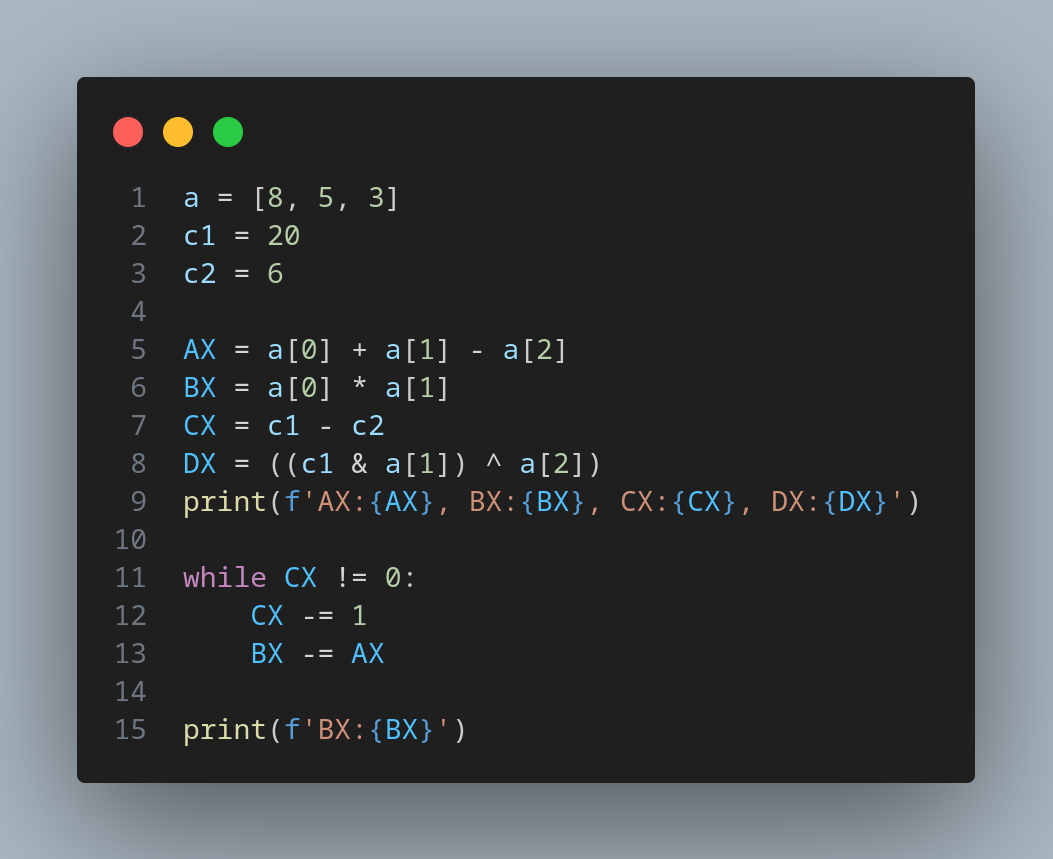
\includegraphics[width=0.8\linewidth]{Prt sc/python_code_1.png}  
        \end{minipage}
    \end{figure}

\newpage
    \begin{center}
        \Large{Results}
    \end{center}
    \begin{figure}[h!]
        \begin{minipage}[h]{1\linewidth}
            \centering
            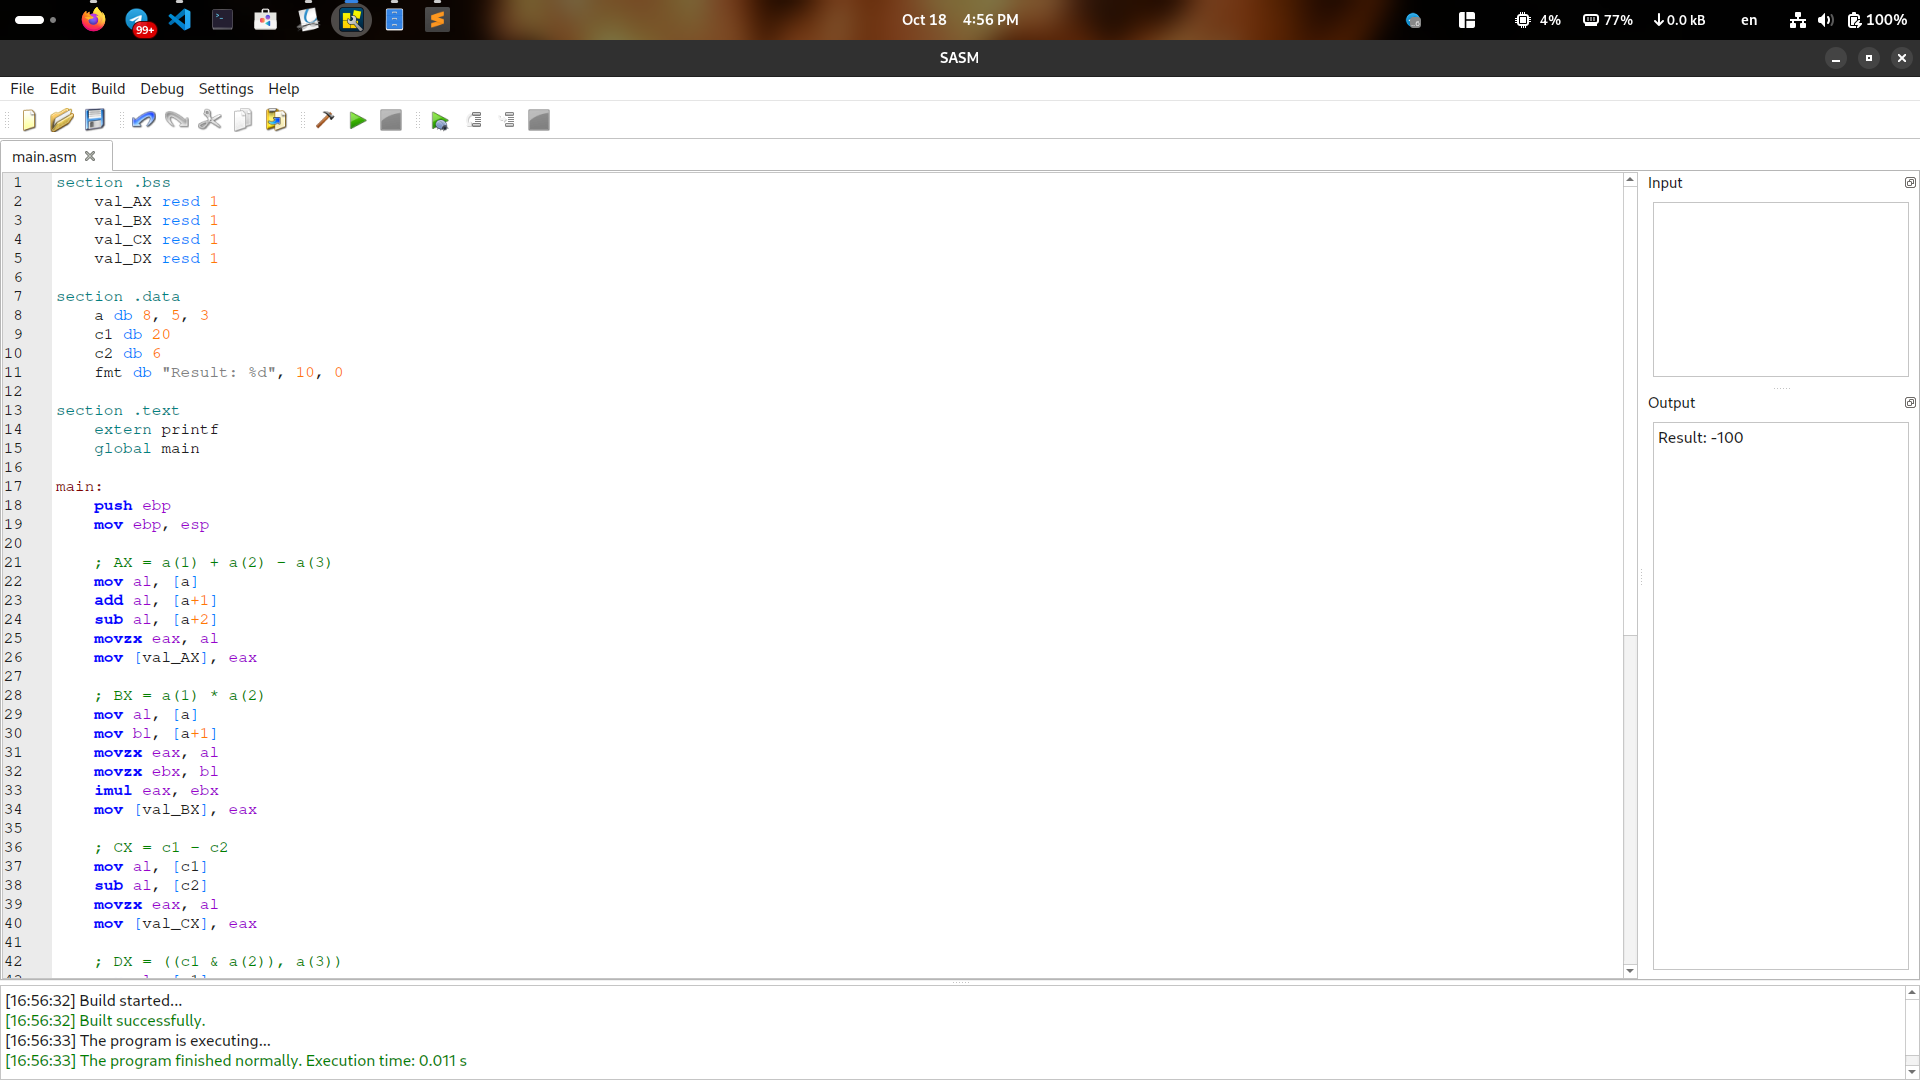
\includegraphics[width=1\linewidth]{Prt sc/1_1.png}  
        \end{minipage}
    \end{figure}
    \begin{figure}[h!]
        \begin{minipage}[h]{1\linewidth}
            \centering
            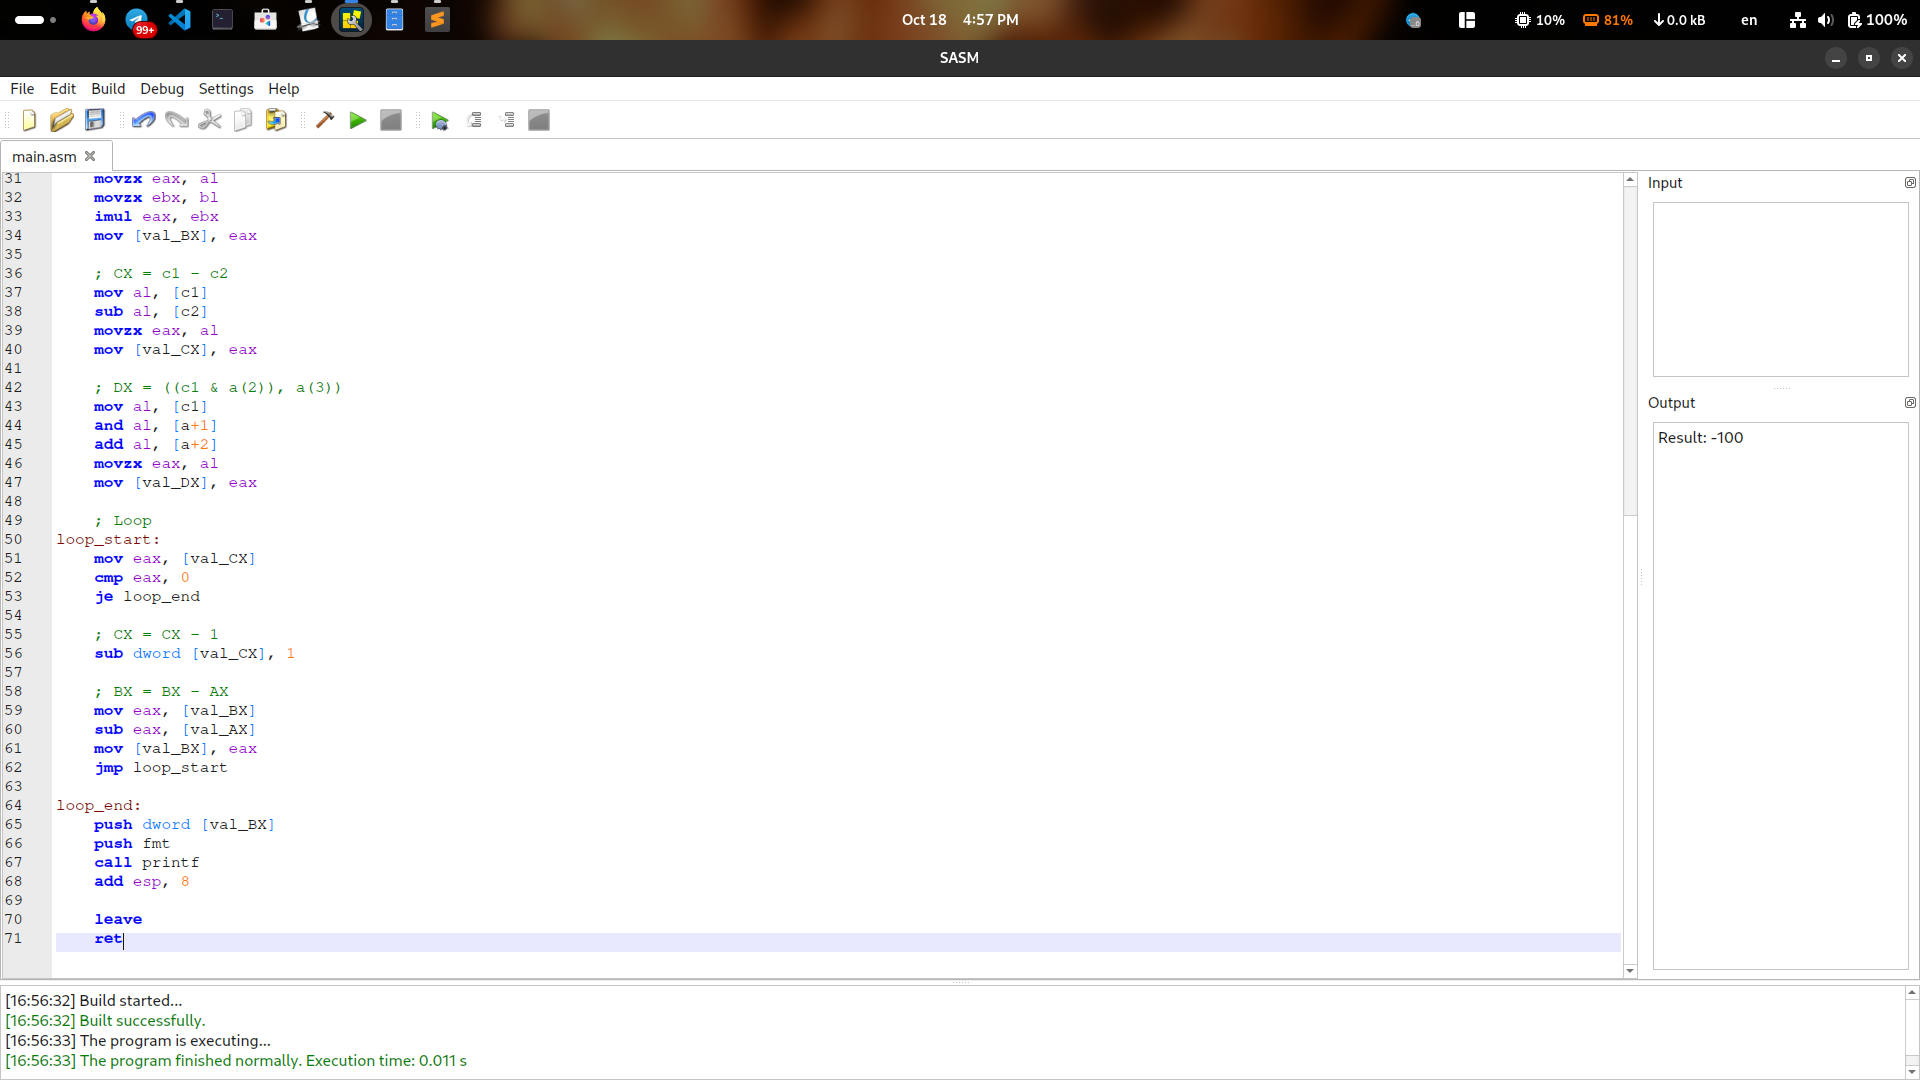
\includegraphics[width=1\linewidth]{Prt sc/1_2.png}  
        \end{minipage}
    \end{figure}

\newpage
    \begin{figure}[h!]
        \begin{minipage}[h]{1\linewidth}
            \centering
            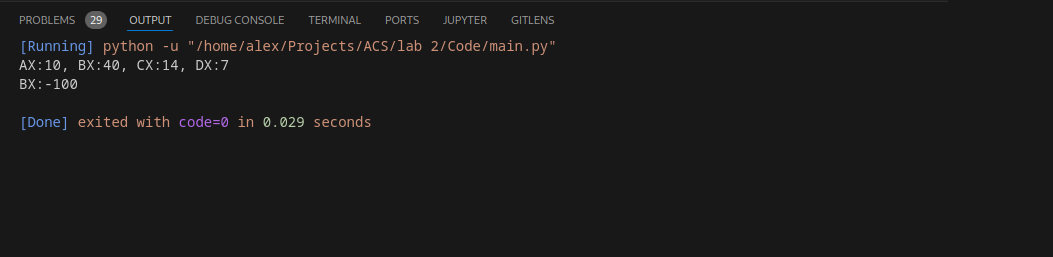
\includegraphics[width=1\linewidth]{Prt sc/python_code_2.png}  
        \end{minipage}
    \end{figure}
    Результати роботи програм співпадають.

\end{document}